\section{ Permutation: n Choose m with Replacement}
The equation for n objects taken m at a time with replacement is
\[{n\choose m} = n^m\]
This is read as "n choose m" with replacement\\
\\
\subsection{Conjecture}
\begin{center}
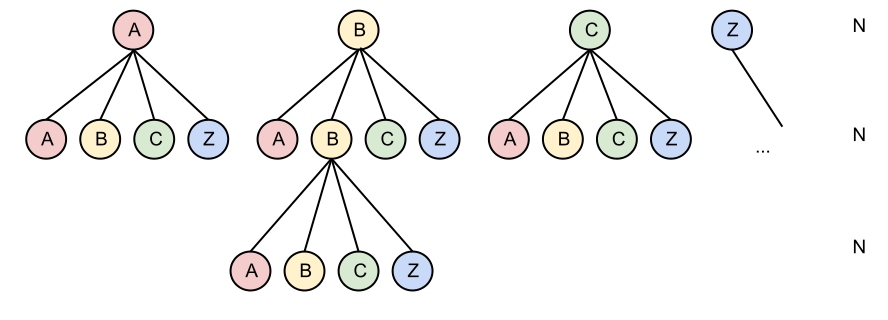
\includegraphics[width=10cm]{Combinatorics/permutations_diag1}
\end{center}
Imagine having N marbles in a bag.  You draw a marble out, then put it back.  The first time you draw there are \(n\) possibilities.  This becomes the first position in your permutation. You have \(n\) different permutations\\
\\
The next time your draw, you have \(n\) possibilities again.  For each of the previous \(n\), they have \(n\) possiblities for the second position.  Now you have \(n\times n = n^2\). \\
\\
This will continue until you have drawn m times
\\
Therefore
\[{n\choose m} = n^m\]


\section{ Permutation: n Choose m with No Replacement}
The equation for n objects taken m at a time without replacement is
\[{n\choose m} = \frac{n!}{(n-m)!}\]
This is read as "n choose m" without replacement\\
\\
\subsection{Conjecture}
\begin{center}
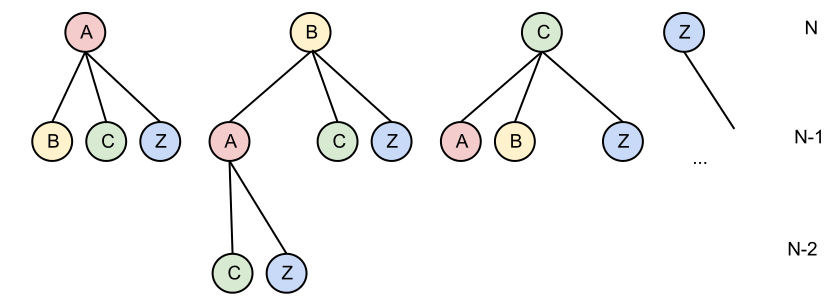
\includegraphics[width=10cm]{Combinatorics/permutations_diag2}
\end{center}
Imagine having N marbles in a bag.  You draw a marble out, but do not put it back in the bag.  The first time you draw there are \(n\) possibilities.  This becomes the first position in your permutation. You have \(n\) different permutations\\
\\
The next time your draw, you have only \(n-1\).  For each of the previous \(n\), they have \(n\) possiblities for the second position.  Now you have \(n\times (n-1)\). \\
\\
The next time your draw, you have \(n-2\).  For each of the previous \(n-1\), they have \(n-2\) possiblities for the third position.  Now you have \(n\times (n-1) \times (n-2) \). \\
If this continued until there were no marbles left, you would have \(n(n-1)(n-2)...(2)(1) = n!\), but you stop after \(m\) times ( where \(m<n\)).  This can be written as:\\
\begin{align*}
{n \choose m} &= \frac{n(n-1)(n-2)...(n-m)(n-m-1)...(2)(1)}{(n-m)(n-m-1)...(2)(1)}\\
{n \choose m} &= \frac{n!}{(n-m)!}
\end{align*}
\\
\section{ Combination: n Choose m with Replacement}
\[{n \choose m} = \frac{n^m}{m!}\]

\subsection{Conjecture}
A Combination is the same as a permutation, but where order is not important.  So ABC, BAC, CBA, and so forth, are all the same.\\
\\
So start with the the equation for permuation with replacement, then we will reduce it by the number of the number of permuations in the sequence. So\\
\[{n \choose m} = n^m\]
With \(m!\) being unique, so\\
\[{n \choose m} = \frac{n^m}{m!}\]

\section{ Combination: n Choose m with No Replacement}
\[{n \choose m} = \frac{n!}{m!(n-m)!}\]

\subsection{Conjecture}
A Combination is the same as a permutation, but where order is not important.  So ABC, BAC, CBA, and so forth, are all the same.\\
\\
So start with the the equation for permuation without replacement, then we will reduce it by the number of the number of permuations in the sequence. So\\
\[{n \choose m} = \frac{n!}{(n-m)!}\]
With \(m!\) being unique, so\\
\[{n \choose m} = \frac{n!}{m!(n-m)!}\]
